\documentclass[3p,times]{amsart}
%\usepackage[margin=1in, bottom=1in, top=1in]{geometry} %1 inch margins
\usepackage{amsmath, amssymb, amstext}
\usepackage{amsthm}
\usepackage{fancyhdr}
\usepackage{algorithm}
\usepackage{algpseudocode}
\usepackage{mathtools}
\usepackage{xcolor}
\usepackage{tikz}
\usepackage{graphicx}
\usepackage{caption}
\usepackage{subcaption}
\usetikzlibrary[topaths]
\usetikzlibrary{decorations.pathmorphing}
\usetikzlibrary{decorations.markings}
\DeclarePairedDelimiter{\ceil}{\lceil}{\rceil}
\DeclarePairedDelimiter\floor{\lfloor}{\rfloor}

%Macros
\newcommand{\A}{\mathbb{A}} \newcommand{\C}{\mathbb{C}}
\newcommand{\D}{\mathbb{D}} \newcommand{\F}{\mathbb{F}}
\newcommand{\N}{\mathbb{N}} \newcommand{\R}{\mathbb{R}}
\newcommand{\T}{\mathbb{T}} \newcommand{\Z}{\mathbb{Z}}
\newcommand{\Q}{\mathbb{Q}}
 
 
\newcommand{\cA}{\mathcal{A}} \newcommand{\cB}{\mathcal{B}}
\newcommand{\cC}{\mathcal{C}} \newcommand{\cD}{\mathcal{D}}
\newcommand{\cE}{\mathcal{E}} \newcommand{\cF}{\mathcal{F}}
\newcommand{\cG}{\mathcal{G}} \newcommand{\cH}{\mathcal{H}}
\newcommand{\cI}{\mathcal{I}} \newcommand{\cJ}{\mathcal{J}}
\newcommand{\cK}{\mathcal{K}} \newcommand{\cL}{\mathcal{L}}
\newcommand{\cM}{\mathcal{M}} \newcommand{\cN}{\mathcal{N}}
\newcommand{\cO}{\mathcal{O}} \newcommand{\cP}{\mathcal{P}}
\newcommand{\cQ}{\mathcal{Q}} \newcommand{\cR}{\mathcal{R}}
\newcommand{\cS}{\mathcal{S}} \newcommand{\cT}{\mathcal{T}}
\newcommand{\cU}{\mathcal{U}} \newcommand{\cV}{\mathcal{V}}
\newcommand{\cW}{\mathcal{W}} \newcommand{\cX}{\mathcal{X}}
\newcommand{\cY}{\mathcal{Y}} \newcommand{\cZ}{\mathcal{Z}}


\DeclareMathOperator{\convOp}{conv}
\newcommand{\conv}{\convOp}

\renewcommand{\thesubfigure}{\Alph{subfigure}}

\newtheorem{claim}{Claim}

\begin{document}

\title{Three Dimensional Stable Matchings with Cyclic Preferences}

\maketitle

In this note, we assume that $n=5$, i.e. we have five men $\mathcal{M}:=\{m_1, \ldots, m_5\}$, five women $\mathcal{W}:=\{w_1, \ldots, w_5\}$ and five dogs $\mathcal{D}:=\{d_1, \ldots, d_5\}$. Each man has a strict preference list over all five women, each woman has a strict preference list over all five dogs, and every dog has a strict preference list over all five men.

For $n=4$, due to the result of Erikkson et.al. we know that there always exists a stable matching. Here, for $n=5$ we are going to try to find an instance $\mathcal{I}$ which does not permit any stable matching.

\section{First Preferences}

\subsection{Forbidden Configurations}
The following configurations for first preferences are not possible in $\mathcal{I}$.

\begin{figure}[H]
	\centering
	\begin{subfigure}{.4\linewidth}
		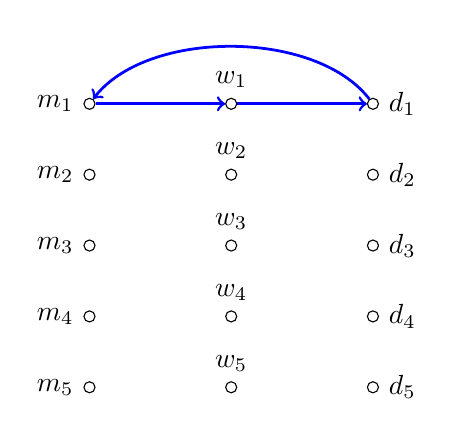
\begin{tikzpicture}[yscale=.9,xscale=1.2]
			\node[shape=circle,draw=black,inner sep=0pt, minimum size=4pt, label=left:$m_1$] (m1) at (0,4) {};
			\node[shape=circle,draw=black,inner sep=0pt, minimum size=4pt, label=above:$w_1$](w1) at (1.5,4){};
			\node[shape=circle,draw=black,inner sep=0pt, minimum size=4pt, label=right:$d_1$](d1) at (3,4){};
			\node[shape=circle,draw=black,inner sep=0pt, minimum size=4pt, label=left:$m_2$] (m2) at (0,3) {};
			\node[shape=circle,draw=black,inner sep=0pt, minimum size=4pt, label=above:$w_2$](w2) at (1.5,3){};
			\node[shape=circle,draw=black,inner sep=0pt, minimum size=4pt, label=right:$d_2$](d2) at (3,3){};
			\node[shape=circle,draw=black,inner sep=0pt, minimum size=4pt, label=left:$m_3$] (m3) at (0,2) {};
			\node[shape=circle,draw=black,inner sep=0pt, minimum size=4pt, label=above:$w_3$](w3) at (1.5,2){};
			\node[shape=circle,draw=black,inner sep=0pt, minimum size=4pt, label=right:$d_3$](d3) at (3,2){};
			\node[shape=circle,draw=black,inner sep=0pt, minimum size=4pt, label=left:$m_4$] (m4) at (0,1) {};
			\node[shape=circle,draw=black,inner sep=0pt, minimum size=4pt, label=above:$w_4$](w4) at (1.5,1){};
			\node[shape=circle,draw=black,inner sep=0pt, minimum size=4pt, label=right:$d_4$](d4) at (3,1){};
			\node[shape=circle,draw=black,inner sep=0pt, minimum size=4pt, label=left:$m_5$] (m5) at (0,0) {};
			\node[shape=circle,draw=black,inner sep=0pt, minimum size=4pt, label=above:$w_5$](w5) at (1.5,0){};
			\node[shape=circle,draw=black,inner sep=0pt, minimum size=4pt, label=right:$d_5$](d5) at (3,0){};

			%% lines
			\draw[->, line width=1pt, blue] (d1) edge[bend right = 60] (m1);
			\draw[->, line width=1pt, blue] (m1) edge (w1);
			\draw[->, line width=1pt, blue] (w1) edge (d1);
		\end{tikzpicture}
		\subcaption{}
		\label{conf: 3 cycle}
	\end{subfigure}
	\hspace{.15\linewidth}
	\begin{subfigure}{.4\linewidth}
		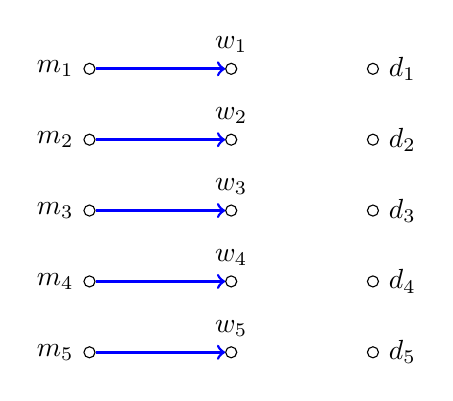
\begin{tikzpicture}[yscale=.9,xscale=1.2]
			\node[shape=circle,draw=black,inner sep=0pt, minimum size=4pt, label=left:$m_1$] (m1) at (0,4) {};
			\node[shape=circle,draw=black,inner sep=0pt, minimum size=4pt, label=above:$w_1$](w1) at (1.5,4){};
			\node[shape=circle,draw=black,inner sep=0pt, minimum size=4pt, label=right:$d_1$](d1) at (3,4){};
			\node[shape=circle,draw=black,inner sep=0pt, minimum size=4pt, label=left:$m_2$] (m2) at (0,3) {};
			\node[shape=circle,draw=black,inner sep=0pt, minimum size=4pt, label=above:$w_2$](w2) at (1.5,3){};
			\node[shape=circle,draw=black,inner sep=0pt, minimum size=4pt, label=right:$d_2$](d2) at (3,3){};
			\node[shape=circle,draw=black,inner sep=0pt, minimum size=4pt, label=left:$m_3$] (m3) at (0,2) {};
			\node[shape=circle,draw=black,inner sep=0pt, minimum size=4pt, label=above:$w_3$](w3) at (1.5,2){};
			\node[shape=circle,draw=black,inner sep=0pt, minimum size=4pt, label=right:$d_3$](d3) at (3,2){};
			\node[shape=circle,draw=black,inner sep=0pt, minimum size=4pt, label=left:$m_4$] (m4) at (0,1) {};
			\node[shape=circle,draw=black,inner sep=0pt, minimum size=4pt, label=above:$w_4$](w4) at (1.5,1){};
			\node[shape=circle,draw=black,inner sep=0pt, minimum size=4pt, label=right:$d_4$](d4) at (3,1){};
			\node[shape=circle,draw=black,inner sep=0pt, minimum size=4pt, label=left:$m_5$] (m5) at (0,0) {};
			\node[shape=circle,draw=black,inner sep=0pt, minimum size=4pt, label=above:$w_5$](w5) at (1.5,0){};
			\node[shape=circle,draw=black,inner sep=0pt, minimum size=4pt, label=right:$d_5$](d5) at (3,0){};

			%% lines
			\draw[->, line width=1pt, blue] (m1) edge (w1);
			\draw[->, line width=1pt, blue] (m2) edge (w2);
			\draw[->, line width=1pt, blue] (m3) edge (w3);
			\draw[->, line width=1pt, blue] (m4) edge (w4);
			\draw[->, line width=1pt, blue] (m5) edge (w5);
		\end{tikzpicture}
		\subcaption{}
		\label{conf: all are prefered}
	\end{subfigure}

	\vspace{.1\linewidth}
	
	\begin{subfigure}{.4\linewidth}
		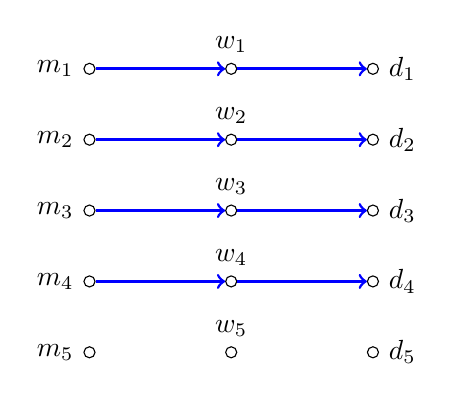
\begin{tikzpicture}[yscale=.9,xscale=1.2]
			\node[shape=circle,draw=black,inner sep=0pt, minimum size=4pt, label=left:$m_1$] (m1) at (0,4) {};
			\node[shape=circle,draw=black,inner sep=0pt, minimum size=4pt, label=above:$w_1$](w1) at (1.5,4){};
			\node[shape=circle,draw=black,inner sep=0pt, minimum size=4pt, label=right:$d_1$](d1) at (3,4){};
			\node[shape=circle,draw=black,inner sep=0pt, minimum size=4pt, label=left:$m_2$] (m2) at (0,3) {};
			\node[shape=circle,draw=black,inner sep=0pt, minimum size=4pt, label=above:$w_2$](w2) at (1.5,3){};
			\node[shape=circle,draw=black,inner sep=0pt, minimum size=4pt, label=right:$d_2$](d2) at (3,3){};
			\node[shape=circle,draw=black,inner sep=0pt, minimum size=4pt, label=left:$m_3$] (m3) at (0,2) {};
			\node[shape=circle,draw=black,inner sep=0pt, minimum size=4pt, label=above:$w_3$](w3) at (1.5,2){};
			\node[shape=circle,draw=black,inner sep=0pt, minimum size=4pt, label=right:$d_3$](d3) at (3,2){};
			\node[shape=circle,draw=black,inner sep=0pt, minimum size=4pt, label=left:$m_4$] (m4) at (0,1) {};
			\node[shape=circle,draw=black,inner sep=0pt, minimum size=4pt, label=above:$w_4$](w4) at (1.5,1){};
			\node[shape=circle,draw=black,inner sep=0pt, minimum size=4pt, label=right:$d_4$](d4) at (3,1){};
			\node[shape=circle,draw=black,inner sep=0pt, minimum size=4pt, label=left:$m_5$] (m5) at (0,0) {};
			\node[shape=circle,draw=black,inner sep=0pt, minimum size=4pt, label=above:$w_5$](w5) at (1.5,0){};
			\node[shape=circle,draw=black,inner sep=0pt, minimum size=4pt, label=right:$d_5$](d5) at (3,0){};

			%% lines
			\draw[->, line width=1pt, blue] (m1) edge (w1);
			\draw[->, line width=1pt, blue] (m2) edge (w2);
			\draw[->, line width=1pt, blue] (m3) edge (w3);
			\draw[->, line width=1pt, blue] (m4) edge (w4);
			\draw[->, line width=1pt, blue] (w1) edge (d1);
			\draw[->, line width=1pt, blue] (w2) edge (d2);
			\draw[->, line width=1pt, blue] (w3) edge (d3);
			\draw[->, line width=1pt, blue] (w4) edge (d4);		
		\end{tikzpicture}
		\subcaption{}
		\label{conf: 4 times 2 are prefered}
	\end{subfigure}	
	\hspace{.15\linewidth}
	\begin{subfigure}{.4\linewidth}
		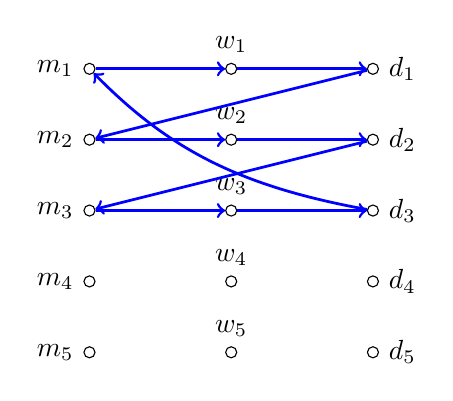
\begin{tikzpicture}[yscale=.9,xscale=1.2]
			\node[shape=circle,draw=black,inner sep=0pt, minimum size=4pt, label=left:$m_1$] (m1) at (0,4) {};
			\node[shape=circle,draw=black,inner sep=0pt, minimum size=4pt, label=above:$w_1$](w1) at (1.5,4){};
			\node[shape=circle,draw=black,inner sep=0pt, minimum size=4pt, label=right:$d_1$](d1) at (3,4){};
			\node[shape=circle,draw=black,inner sep=0pt, minimum size=4pt, label=left:$m_2$] (m2) at (0,3) {};
			\node[shape=circle,draw=black,inner sep=0pt, minimum size=4pt, label=above:$w_2$](w2) at (1.5,3){};
			\node[shape=circle,draw=black,inner sep=0pt, minimum size=4pt, label=right:$d_2$](d2) at (3,3){};
			\node[shape=circle,draw=black,inner sep=0pt, minimum size=4pt, label=left:$m_3$] (m3) at (0,2) {};
			\node[shape=circle,draw=black,inner sep=0pt, minimum size=4pt, label=above:$w_3$](w3) at (1.5,2){};
			\node[shape=circle,draw=black,inner sep=0pt, minimum size=4pt, label=right:$d_3$](d3) at (3,2){};
			\node[shape=circle,draw=black,inner sep=0pt, minimum size=4pt, label=left:$m_4$] (m4) at (0,1) {};
			\node[shape=circle,draw=black,inner sep=0pt, minimum size=4pt, label=above:$w_4$](w4) at (1.5,1){};
			\node[shape=circle,draw=black,inner sep=0pt, minimum size=4pt, label=right:$d_4$](d4) at (3,1){};
			\node[shape=circle,draw=black,inner sep=0pt, minimum size=4pt, label=left:$m_5$] (m5) at (0,0) {};
			\node[shape=circle,draw=black,inner sep=0pt, minimum size=4pt, label=above:$w_5$](w5) at (1.5,0){};
			\node[shape=circle,draw=black,inner sep=0pt, minimum size=4pt, label=right:$d_5$](d5) at (3,0){};

			%% lines
			\draw[->, line width=1pt, blue] (m1) edge (w1);
			\draw[->, line width=1pt, blue] (w1) edge (d1);
			\draw[->, line width=1pt, blue] (d1) edge (m2);
			\draw[->, line width=1pt, blue] (m2) edge (w2);
			\draw[->, line width=1pt, blue] (w2) edge (d2);
			\draw[->, line width=1pt, blue] (d2) edge (m3);
			\draw[->, line width=1pt, blue] (m3) edge (w3);
			\draw[->, line width=1pt, blue] (w3) edge (d3);
			\draw[->, line width=1pt, blue] (d3) edge[bend left = 20] (m1);
		\end{tikzpicture}
		\subcaption{}
		\label{conf: 9 cycle}
	\end{subfigure}	
	\caption{Forbidden configurations for first preferences.}
\end{figure}

\smallskip

The configurations~\ref{conf: 3 cycle} and ~\ref{conf: all are prefered} are clearly forbidden for $\mathcal{I}$.

\smallskip

The configurations~\ref{conf: 4 times 2 are prefered} is forbidden, since $\{m_i,w_i, d_i\}$, $i=1,\ldots,5$ is a stable matching in this case.

\smallskip

The configuration~\ref{conf: 9 cycle} is forbidden as well. Indeed, assume that $w_4>_{m_4} w_5$ and $w_5>_{m_5} w_4$. Then, $\{m_i,w_i, d_i\}$, $i=1,\ldots,5$ is a stable matching. Thus, with respect to symmetry we may assume that
\begin{align*}
	&w_4>_{m_4} w_5\,,\qquad w_4>_{m_5} w_5\\
	&d_4>_{w_4} d_5\,,\qquad d_4>_{w_5} d_5\\
	&m_4>_{d_4} m_5\,,\qquad m_4>_{d_5} d_5\,.\\
\end{align*}
In this case, $\{m_i,w_i, d_i\}$, $i=1,\ldots,5$ is a stable matching. 

\bigskip
\subsection{Start}
The forbidden configurations~\ref{conf: 3 cycle} and ~\ref{conf: all are prefered} imply that we can start with the preferences in Figure~\ref{fig:start}, where the red circles mark the men, women and dogs which can never be first in the preference list.

\begin{figure}[H]
	\centering
		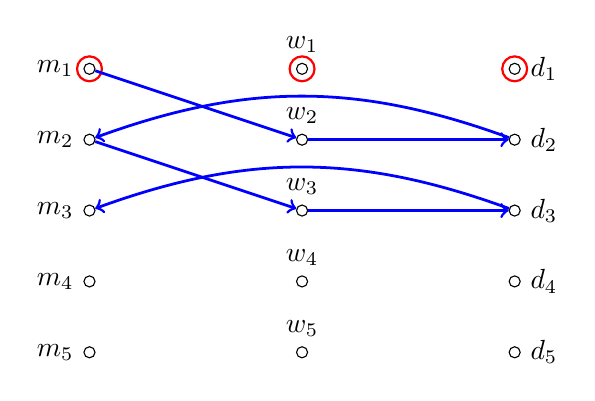
\begin{tikzpicture}[yscale=.9,xscale=.9]
			\node[shape=circle,draw=black,inner sep=0pt, minimum size=4pt, label=left:$m_1$] (m1) at (0,4) {};
			\node[shape=circle,draw=black,inner sep=0pt, minimum size=4pt, label=above:$w_1$](w1) at (3,4){};
			\node[shape=circle,draw=black,inner sep=0pt, minimum size=4pt, label=right:$d_1$](d1) at (6,4){};
			\node[shape=circle,draw=black,inner sep=0pt, minimum size=4pt, label=left:$m_2$] (m2) at (0,3) {};
			\node[shape=circle,draw=black,inner sep=0pt, minimum size=4pt, label=above:$w_2$](w2) at (3,3){};
			\node[shape=circle,draw=black,inner sep=0pt, minimum size=4pt, label=right:$d_2$](d2) at (6,3){};
			\node[shape=circle,draw=black,inner sep=0pt, minimum size=4pt, label=left:$m_3$] (m3) at (0,2) {};
			\node[shape=circle,draw=black,inner sep=0pt, minimum size=4pt, label=above:$w_3$](w3) at (3,2){};
			\node[shape=circle,draw=black,inner sep=0pt, minimum size=4pt, label=right:$d_3$](d3) at (6,2){};
			\node[shape=circle,draw=black,inner sep=0pt, minimum size=4pt, label=left:$m_4$] (m4) at (0,1) {};
			\node[shape=circle,draw=black,inner sep=0pt, minimum size=4pt, label=above:$w_4$](w4) at (3,1){};
			\node[shape=circle,draw=black,inner sep=0pt, minimum size=4pt, label=right:$d_4$](d4) at (6,1){};
			\node[shape=circle,draw=black,inner sep=0pt, minimum size=4pt, label=left:$m_5$] (m5) at (0,0) {};
			\node[shape=circle,draw=black,inner sep=0pt, minimum size=4pt, label=above:$w_5$](w5) at (3,0){};
			\node[shape=circle,draw=black,inner sep=0pt, minimum size=4pt, label=right:$d_5$](d5) at (6,0){};
			%% circles
			\draw[red,thick] (m1) circle (5pt);
			\draw[red,thick] (w1) circle (5pt);
			\draw[red,thick] (d1) circle (5pt);
			%% lines
			\draw[->, line width=1pt, blue] (m1) edge (w2);
			\draw[->, line width=1pt, blue] (w2) edge (d2);
			\draw[->, line width=1pt, blue] (d2) edge[bend right= 20]  (m2);
			\draw[->, line width=1pt, blue] (m2) edge (w3);
			\draw[->, line width=1pt, blue] (w3) edge (d3);
			\draw[->, line width=1pt, blue] (d3) edge[bend right= 20]  (m3);
		\end{tikzpicture}
	\caption{Starting preference.}
	\label{fig:start}
\end{figure}

\section{Stable Matchings for Partial Preference Lists}

Assume that 
\begin{enumerate}
\item for each man $m_i\in \mathcal{M}$, $i=1, \ldots, 5$ we know his most preferred $\alpha_i$ women and his preference for these $\alpha_i$ women

\item for each woman $w_i\in \mathcal{W}$, $i=1, \ldots, 5$ we know her most preferred $\beta_i$ dogs and her preference for these $\beta_i$ dogs

\item for each dog $d_i\in \mathcal{D}$, $i=1, \ldots, 5$ we know its most preferred $\gamma_i$ men and its preference for these $\gamma_i$ men.
\end{enumerate}

Thus, we may speak of a new instance $\mathcal{J}$, which represents "partial information" about the instance $\mathcal{I}$.

\bigskip
\begin{claim}
If there is a nonempty stable matching $M$ in $\mathcal{J}$ so that for every $\{m_i, w_j, d_k\}\in M$
\begin{enumerate}
\item for every $w_t$, $w_t >_{m_i} w_j$ the woman $w_t$ is matched by $M$

\item for every $d_t$, $d_t >_{w_j} d_k$ the dog $d_k$ is matched by $M$

\item for every $m_t$, $m_t >_{d_k} m_i$ the man $m_t$ is matched by $M$,
\end{enumerate}
then $\mathcal{I}$ has  a stable matching. 
\end{claim}
\begin{proof}
Indeed, we can take $M$ together with a stable matching for the instance corresponding to $\mathcal{I}$ with deleted men, women and dogs that are matched by $M$.
\end{proof}


\end{document}
